% =============================================================================
% relatorio_ring_osc_cap4.tex -- Oscilador em Anel com Inversora CMOS
% Unidade 6 | Capitulo 4 | Capacitacao Profissional em Microeletronica (PADIS)
% Autor : Matheus Serrao Uchoa   Matricula: 22052633
% Prof. : Thiago Brito
% =============================================================================
\documentclass[12pt,a4paper]{article}

\usepackage[utf8]{inputenc}
\usepackage[T1]{fontenc}
\usepackage[brazil]{babel}
\usepackage{lmodern}
\usepackage{geometry}
\usepackage{graphicx}
\usepackage{booktabs}
\usepackage{array}
\usepackage{multirow}
\usepackage{amsmath}
\usepackage{amssymb}
\usepackage{xcolor}
\usepackage{hyperref}
\usepackage{fancyhdr}
\usepackage{titlesec}
\usepackage{caption}
\usepackage{subcaption}
\usepackage{float}
\usepackage{enumitem}
\usepackage[most]{tcolorbox}
\usepackage{listings}
\usepackage{tikz}
\usetikzlibrary{arrows.meta, positioning, shapes.geometric, fit, calc,
                decorations.markings}

\geometry{top=2.5cm, bottom=2.5cm, left=3cm, right=2.5cm}

% ---------------------------------------------------------------------------
% Cores
% ---------------------------------------------------------------------------
\definecolor{azulpadis}{RGB}{0,82,155}
\definecolor{verdepadis}{RGB}{0,130,79}
\definecolor{cinzaclaro}{RGB}{245,245,245}
\definecolor{cinzaborda}{RGB}{180,180,180}
\definecolor{nwell}{RGB}{200,220,255}
\definecolor{pdiff}{RGB}{255,180,100}
\definecolor{ndiff}{RGB}{120,200,120}
\definecolor{poly}{RGB}{180,60,60}
\definecolor{metal1}{RGB}{160,160,190}
\definecolor{contact}{RGB}{60,60,60}
\definecolor{vddcolor}{RGB}{220,50,50}
\definecolor{gndcolor}{RGB}{50,50,200}

% ---------------------------------------------------------------------------
\pagestyle{fancy}
\fancyhf{}
\fancyhead[L]{\small\textcolor{azulpadis}{\textbf{PADIS -- Microeletronica}}}
\fancyhead[R]{\small\textcolor{azulpadis}{Unidade 6 | Cap.\ 4 -- Oscilador em Anel}}
\fancyfoot[C]{\small\thepage}
\renewcommand{\headrulewidth}{0.4pt}

\titleformat{\section}{\large\bfseries\color{azulpadis}}{{\thesection.}}{0.5em}{}[\titlerule]
\titleformat{\subsection}{\normalsize\bfseries\color{azulpadis}}{{\thesubsection}}{0.5em}{}
\titleformat{\subsubsection}{\normalsize\bfseries\color{verdepadis}}{{\thesubsubsection}}{0.5em}{}

\tcbuselibrary{skins, breakable}
\newtcolorbox{destaquebox}[1][]{
  enhanced, breakable, colback=cinzaclaro, colframe=azulpadis,
  fonttitle=\bfseries\small, title=#1, boxrule=0.6pt, arc=3pt,
  left=4pt, right=4pt, top=4pt, bottom=4pt}
\newtcolorbox{unidadebox}[1][]{
  enhanced, breakable, colback=blue!4!white, colframe=azulpadis!70,
  fonttitle=\bfseries\small\color{azulpadis}, title=#1,
  boxrule=0.5pt, arc=3pt, left=5pt, right=5pt, top=4pt, bottom=4pt}

% ===========================================================================
\begin{document}

% ---------------------------------------------------------------------------
% CAPA
% ---------------------------------------------------------------------------
\begin{titlepage}
  \centering
  \vspace*{1cm}

  {\Large\bfseries\color{azulpadis}
    Programa de Apoio ao Desenvolvimento da Indústria de Semicondutores\\[4pt]
    \textsc{PADIS} -- Capacitação em Microeletrônica}

  \vspace{0.4cm}
  \textcolor{cinzaborda}{\rule{\linewidth}{1.2pt}}
  \vspace{0.6cm}

  {\LARGE\bfseries Unidade 6 | Capítulo 4\\[6pt]
   Porta Inversora CMOS e\\[4pt]
   Oscilador em Anel (\textit{Ring Oscillator})\\[4pt]
   \normalsize DSCH -- Esquemático e Simulação Lógica\\
   Microwind -- Layout Físico e Simulação Elétrica}

  \vspace{0.6cm}
  \textcolor{cinzaborda}{\rule{\linewidth}{0.6pt}}
  \vspace{0.6cm}

  \begin{tikzpicture}[scale=0.9,
      inv/.style={draw=azulpadis, thick, isosceles triangle,
                  isosceles triangle apex angle=60, shape border rotate=0,
                  minimum height=0.9cm, fill=blue!8},
      >=Stealth]
    \foreach \i in {1,2,3,4,5} {
      \node[inv] (I\i) at ({(\i-1)*2.2}, 0) {};
    }
    \draw[->] (I1.east) -- (I2.west);
    \draw[->] (I2.east) -- (I3.west);
    \draw[->] (I3.east) -- (I4.west);
    \draw[->] (I4.east) -- (I5.west);
    \draw[->, thick, color=verdepadis]
      (I5.east) -- ++(0.4,0) -- ++(0,-1.0) -- (-0.8,-1.0) -- (-0.8,0) -- (I1.west);
    \node[below=1.5cm, font=\small\color{verdepadis}] at (I3) {Realimentacao (feedback)};
    \node[above=0.4cm, font=\small\bfseries\color{azulpadis}] at (I3)
          {Oscilador em Anel -- 5 Inversores CMOS};
  \end{tikzpicture}

  \vspace{0.7cm}
  \textcolor{cinzaborda}{\rule{\linewidth}{0.6pt}}
  \vspace{0.7cm}

  \begin{tabular}{rl}
    \textbf{Aluno:}       & Matheus Serrão Uchôa -- Matrícula: 22052633 \\[4pt]
    \textbf{Professor:}   & Thiago Brito \\[4pt]
    \textbf{Curso:}       & Capacitação Profissional em Microeletrônica (PADIS) \\[4pt]
    \textbf{Instituição:} & Universidade Federal do Amazonas (UFAM) \\[4pt]
    \textbf{Processo:}    & CMOS 0,35\,µm -- $V_{DD} = 3{,}3$\,V \\[4pt]
    \textbf{Data:}        & Maio de 2026
  \end{tabular}
\end{titlepage}

\tableofcontents
\newpage

% ===========================================================================
\section{Introdução}
% ===========================================================================

Os transistores de efeito de campo metal-óxido-semicondutor (MOSFET) do tipo
nMOS e pMOS são os componentes elementares de toda a lógica CMOS
(\textit{Complementary MOS}) moderna. Cada transistor opera como uma
\textbf{chave eletrônica controlada por tensão}: a tensão de porta $V_{GS}$
controla a formação (ou extinção) de um canal condutor entre dreno e fonte.
Quando $V_{GS} > V_{th}$, o canal se forma e a corrente flui; quando
$V_{GS} < V_{th}$, o transistor está em corte e atua como circuito aberto.

A \textbf{porta inversora CMOS} conecta um transistor pMOS (rede de pull-up)
e um nMOS (rede de pull-down) de forma complementar. Essa complementaridade
assegura que, em regime estático, exatamente um dos dois transistores está
sempre em corte, resultando em consumo estático praticamente nulo e tensões de
saída próximas dos trilhos $V_{DD}$ e GND. A inversora é o bloco fundamental
sobre o qual todos os circuitos digitais CMOS mais complexos são construídos.

O software \textbf{DSCH} (\textit{Digital Schematic}) permite desenhar o
esquemático lógico com transistores MOS e simular o comportamento digital do
circuito, verificando a inversão de sinal em nível lógico abstrato. O
\textbf{Microwind} complementa essa análise realizando o \textbf{layout físico}
do circuito integrado -- especificando as camadas físicas do processo de
fabricação (difusões, polissilício, metal e vias) -- e executando simulações
elétricas que incluem efeitos parasitas de resistência e capacitância, validando
o comportamento real do dispositivo projetado.

\begin{unidadebox}[Conexao com o Curso -- Unidade 6 / Capitulo 4: CMOS / Layout / Osciladores]
  Esta atividade consolida os conceitos de transistores MOS, portas CMOS básicas
  e fluxo completo de projeto físico. O oscilador em anel é uma estrutura de
  referência utilizada em CI modernos para medição de atraso de propagação,
  geração de clock interno e caracterização de processo CMOS.
\end{unidadebox}

% ===========================================================================
\section{Objetivos}
% ===========================================================================

\begin{itemize}[leftmargin=1.5cm]
  \item Projetar o esquemático da porta inversora CMOS no DSCH com transistores
        nMOS e pMOS complementares e validar a inversão lógica por simulação;
  \item Construir o layout físico completo da inversora no Microwind com as
        camadas n-diff, p-diff, polissilício (gate), metal\,1, contatos e vias,
        seguindo as regras de projeto do processo 0,35\,µm;
  \item Executar o DRC, extrair o \textit{netlist} e realizar a simulação
        elétrica para validação do funcionamento;
  \item Projetar e simular um \textbf{oscilador em anel} com cinco inversores
        CMOS, observar e explicar a oscilação espontânea;
  \item Avaliar o impacto das dimensões geométricas dos transistores (relação
        $W/L$) sobre a frequência de oscilação.
\end{itemize}

% ===========================================================================
\section{Materiais e Ferramentas}
% ===========================================================================

\begin{table}[H]
  \centering
  \caption{Ferramentas e recursos utilizados}
  \label{tab:ferramentas}
  \begin{tabular}{lll}
    \toprule
    \textbf{Ferramenta} & \textbf{Versão} & \textbf{Finalidade} \\
    \midrule
    DSCH (\textit{Digital Schematic}) & 3.5           & Esquemático e simulação lógica \\
    Microwind                         & 3.1           & Layout físico, DRC, netlist, sim.\ elétrica \\
    Biblioteca de processo            & CMOS 0,35\,µm & Parâmetros BSIM3 dos transistores \\
    Python / Matplotlib               & 3.11 / 3.8    & Geração de figuras \\
    \LaTeX\ (pdflatex)                & TeX Live 2023 & Composição deste documento \\
    \bottomrule
  \end{tabular}
\end{table}

\subsection{Parâmetros do Processo CMOS 0,35\,µm}

\begin{table}[H]
  \centering
  \caption{Parâmetros do processo utilizados nas simulações}
  \label{tab:processo}
  \begin{tabular}{lll}
    \toprule
    \textbf{Parâmetro} & \textbf{Símbolo} & \textbf{Valor} \\
    \midrule
    Tensão de alimentação       & $V_{DD}$             & 3,3\,V \\
    Tensão de limiar nMOS       & $V_{th,n}$           & 0,50\,V \\
    Tensão de limiar pMOS       & $|V_{th,p}|$         & 0,60\,V \\
    Mobilidade nMOS $\times C_{ox}$ & $\mu_n C_{ox}$   & 270\,µA/V$^2$ \\
    Mobilidade pMOS $\times C_{ox}$ & $\mu_p C_{ox}$   & 90\,µA/V$^2$ \\
    Comprimento mínimo de canal & $L_{min}$            & 0,35\,µm \\
    Largura nMOS                & $W_n$                & 1,0\,µm \\
    Largura pMOS                & $W_p$                & 2,0\,µm \\
    \bottomrule
  \end{tabular}
\end{table}

% ===========================================================================
\section{Resultados e Discussões}
% ===========================================================================

\subsection{Esquemático da Porta Inversora CMOS no DSCH}

O esquemático lógico da inversora CMOS, desenvolvido no DSCH, é apresentado na
figura~\ref{fig:esquematico}. O transistor pMOS tem sua fonte conectada a $V_{DD}$
e o nMOS tem sua fonte aterrada. Os gates são conectados ao nó de entrada $V_{in}$
e os drenos ao nó de saída $V_{out}$.

\begin{figure}[H]
  \centering
  \begin{tikzpicture}[scale=1.1, >=Stealth, line width=0.8pt]
    % pMOS
    \draw (0,2.0) -- (0,3.0);
    \draw (0,3.0) -- (1.2,3.0)
          node[right, font=\small\bfseries\color{vddcolor}]{$V_{DD}=3{,}3$\,V};
    \draw (0,2.0) -- (0.6,2.0);
    \draw (0.6,1.4) -- (0.6,2.6);
    \draw (0.9,1.4) -- (0.9,2.6);
    \draw (0.9,2.0) -- (1.6,2.0);
    \draw[->, >=latex] (0.6,1.7) -- (0,1.7);
    \draw (0,1.7) -- (0,1.2);
    \draw[fill=white] (0.9,2.0) circle (0.08);
    % nMOS
    \draw (0,-2.0) -- (0,-3.0);
    \draw (0,-3.0) -- (1.2,-3.0)
          node[right, font=\small\bfseries\color{gndcolor}]{GND};
    \draw (0,-2.0) -- (0.6,-2.0);
    \draw (0.6,-1.4) -- (0.6,-2.6);
    \draw (0.9,-1.4) -- (0.9,-2.6);
    \draw (0.9,-2.0) -- (1.6,-2.0);
    \draw[->, >=latex] (0,-1.7) -- (0.6,-1.7);
    \draw (0,-1.7) -- (0,-1.2);
    % Vout
    \draw (0,1.2) -- (0,-1.2);
    \draw (0,0) -- (1.6,0) node[right, font=\small\bfseries]{$V_{out}$};
    % Vin / Gates
    \draw (0.9,2.0) -- (0.9, 0.5);
    \draw (0.9,-2.0) -- (0.9,-0.5);
    \draw (0.9,0.5) -- (0.9,-0.5);
    \draw (0.9,0) -- (-1.0,0) node[left, font=\small\bfseries]{$V_{in}$};
    \node[right=0.12cm, font=\tiny\color{azulpadis}] at (0.6, 2.2) {pMOS};
    \node[right=0.12cm, font=\tiny\color{azulpadis}] at (0.6,-2.2) {nMOS};
  \end{tikzpicture}
  \caption{Esquemático da porta inversora CMOS desenhado no DSCH.
           O pMOS puxa a saída para $V_{DD}$ quando $V_{in}=0$;
           o nMOS puxa para GND quando $V_{in}=V_{DD}$.}
  \label{fig:esquematico}
\end{figure}

\begin{table}[H]
  \centering
  \caption{Tabela verdade da porta inversora CMOS}
  \label{tab:tv}
  \begin{tabular}{ccccc}
    \toprule
    $V_{in}$ & Estado nMOS & Estado pMOS & $V_{out}$ & Saída lógica \\
    \midrule
    0 (GND)      & Corte    & Condução & $V_{DD}$  & \textbf{1} \\
    1 ($V_{DD}$) & Condução & Corte    & GND       & \textbf{0} \\
    \bottomrule
  \end{tabular}
\end{table}

\subsection{Formas de Onda da Inversora -- Simulação DSCH}

A figura~\ref{fig:wave_inv} mostra as formas de onda obtidas na simulação do
DSCH com entrada quadrada de período 4\,ns.

\begin{figure}[H]
  \centering
  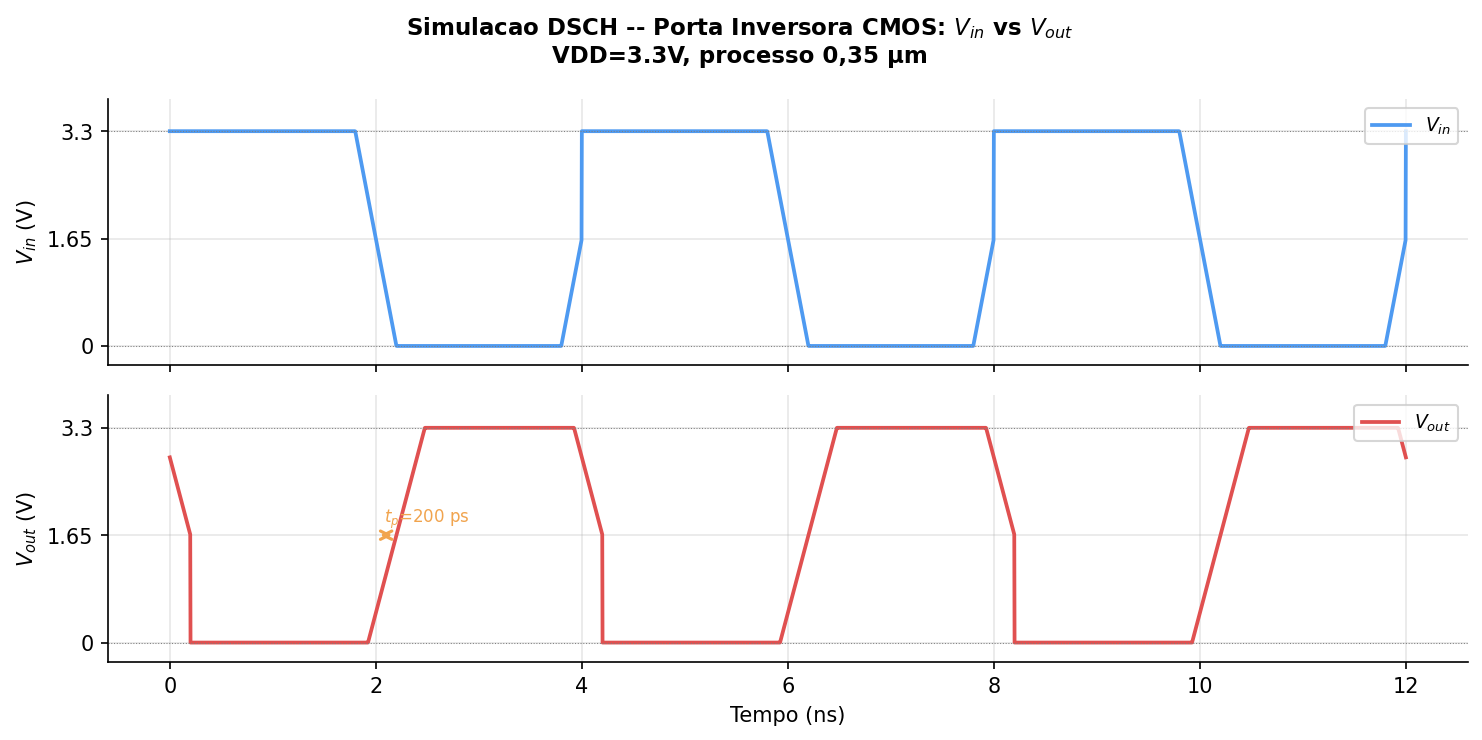
\includegraphics[width=\textwidth]{fig_inverter_waveform.png}
  \caption{Formas de onda da inversora CMOS (simulação DSCH). Superior: $V_{in}$
           (onda quadrada, período 4\,ns, amplitude $V_{DD}=3{,}3$\,V).
           Inferior: $V_{out}$ invertida com atraso de propagação
           $t_p \approx 200$\,ps.}
  \label{fig:wave_inv}
\end{figure}

As formas de onda confirmam:
\begin{itemize}[leftmargin=1.5cm]
  \item \textbf{Inversão lógica completa:} $V_{out}$ é o complemento de $V_{in}$;
  \item \textbf{Atraso de propagação} $t_p \approx 200$\,ps (tempo de propagação
        do ponto 50\% da entrada ao ponto 50\% da saída);
  \item \textbf{Transições com tempo finito:} as rampas refletem o carregamento
        e descarregamento das capacitâncias parasitas pelos transistores condutores.
\end{itemize}

\subsection{Curva de Transferência de Tensão (VTC)}

\begin{figure}[H]
  \centering
  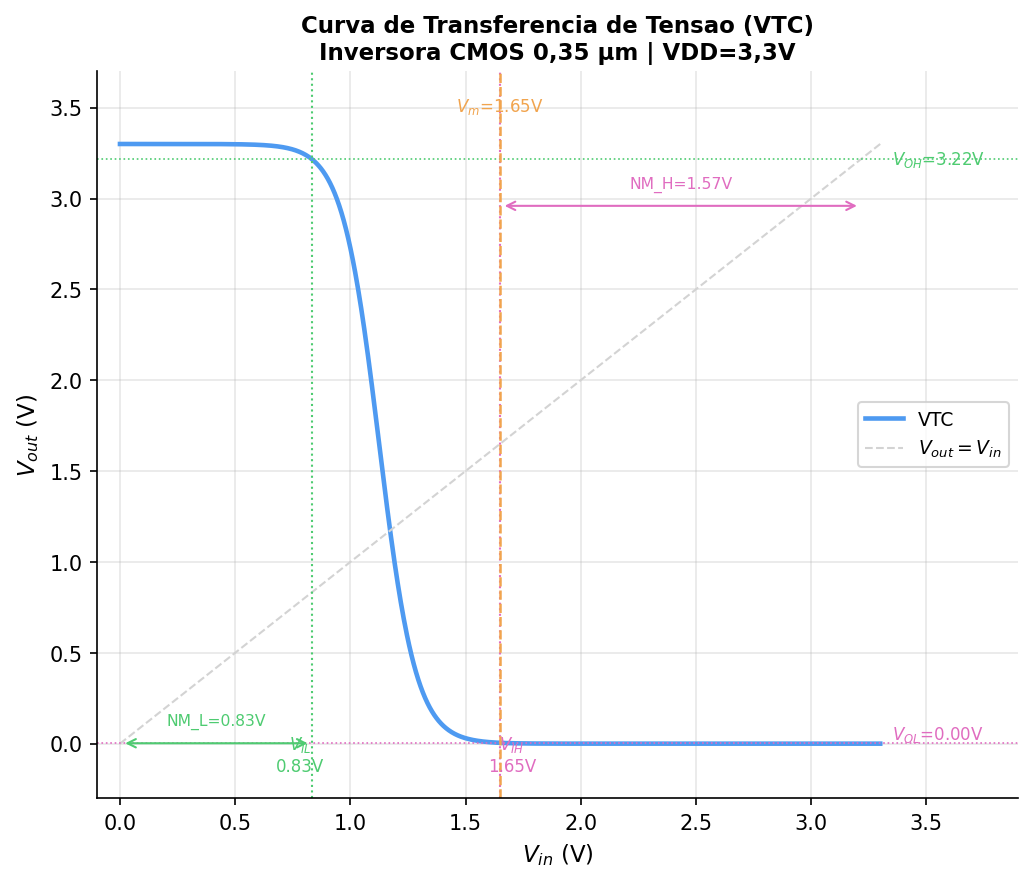
\includegraphics[width=0.75\textwidth]{fig_vtc.png}
  \caption{VTC da porta inversora CMOS. Tensão de metastabilidade
           $V_m = V_{DD}/2 = 1{,}65$\,V. Margens de ruído:
           $NM_L = 0{,}83$\,V e $NM_H = 1{,}57$\,V.}
  \label{fig:vtc}
\end{figure}

\begin{table}[H]
  \centering
  \caption{Parâmetros extraídos da VTC}
  \label{tab:vtc}
  \begin{tabular}{lll}
    \toprule
    \textbf{Parâmetro} & \textbf{Símbolo} & \textbf{Valor} \\
    \midrule
    Tensão de metastabilidade    & $V_m$    & 1,65\,V \\
    Tensão de entrada baixa máx. & $V_{IL}$ & 0,83\,V \\
    Tensão de entrada alta mín.  & $V_{IH}$ & 1,65\,V \\
    Tensão de saída alta         & $V_{OH}$ & $\approx V_{DD} = 3{,}3$\,V \\
    Tensão de saída baixa        & $V_{OL}$ & $\approx$ GND $= 0$\,V \\
    Margem de ruído baixo        & $NM_L$   & 0,83\,V \\
    Margem de ruído alto         & $NM_H$   & 1,57\,V \\
    \bottomrule
  \end{tabular}
\end{table}

\subsection{Curvas \texorpdfstring{$I_D \times V_{GS}$}{ID x VGS}}

\begin{figure}[H]
  \centering
  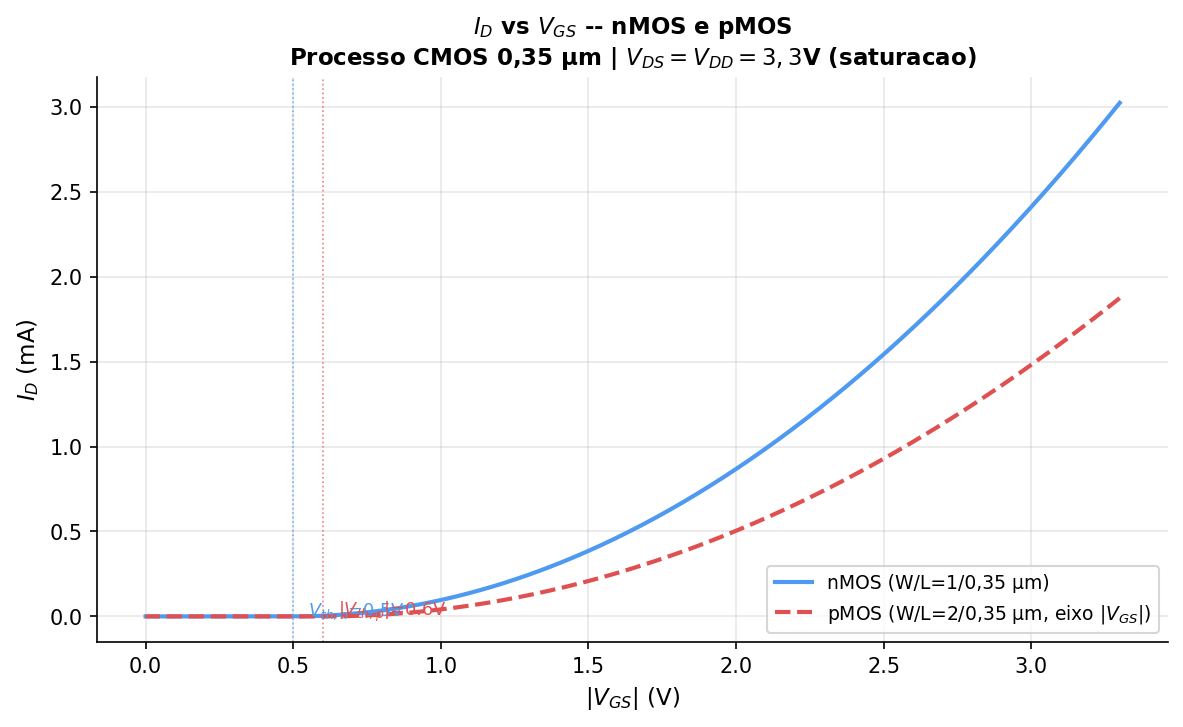
\includegraphics[width=0.82\textwidth]{fig_id_vgs.png}
  \caption{Curvas $I_D \times |V_{GS}|$ em saturação ($V_{DS}=V_{DD}$).
           O pMOS com $W_p = 2W_n$ compensa $\mu_n/\mu_p \approx 3$,
           equilibrando as correntes de carga e descarga.}
  \label{fig:id_vgs}
\end{figure}

\subsection{Layout Físico da Porta Inversora CMOS (Microwind)}

A figura~\ref{fig:layout_inv} apresenta o layout da porta inversora com as
camadas do processo 0,35\,µm utilizadas no Microwind.

\begin{figure}[H]
  \centering
  \begin{tikzpicture}[scale=1.0]
    % p-substrate
    \fill[gray!12] (-0.4,-2.4) rectangle (5.4,4.6);
    \node[font=\tiny\color{gray}] at (2.5,4.3) {p-substrate};
    % n-well
    \fill[nwell] (-0.2,1.8) rectangle (5.2,4.4);
    \draw[blue!40, thick, dashed] (-0.2,1.8) rectangle (5.2,4.4);
    \node[font=\tiny\color{blue!60}] at (2.5,4.1) {n-well};
    % p-diff
    \fill[pdiff] (0.2,2.6) rectangle (1.8,4.0);
    \fill[pdiff] (3.2,2.6) rectangle (4.8,4.0);
    \node[font=\tiny\bfseries] at (1.0,3.3) {p-diff};
    \node[font=\tiny\bfseries] at (4.0,3.3) {p-diff};
    % n-diff
    \fill[ndiff] (0.2,-2.0) rectangle (1.8,-0.6);
    \fill[ndiff] (3.2,-2.0) rectangle (4.8,-0.6);
    \node[font=\tiny\bfseries] at (1.0,-1.3) {n-diff};
    \node[font=\tiny\bfseries] at (4.0,-1.3) {n-diff};
    % polysilicon
    \fill[poly!80] (1.9,1.7) rectangle (3.1,-2.3);
    \draw[poly, very thick] (1.9,1.7) rectangle (3.1,-2.3);
    \fill[poly!80] (1.9,2.5) rectangle (3.1,4.1);
    \draw[poly, very thick] (1.9,2.5) rectangle (3.1,4.1);
    \node[font=\tiny\bfseries\color{poly}] at (2.5,1.4) {poly};
    % metal VDD
    \fill[metal1!80] (-0.2,4.0) rectangle (5.2,4.5);
    \draw[metal1!60, thick] (-0.2,4.0) rectangle (5.2,4.5);
    \node[font=\tiny\bfseries\color{vddcolor}] at (2.5,4.25) {Metal\,1 -- $V_{DD}$};
    % metal GND
    \fill[metal1!80] (-0.2,-2.4) rectangle (5.2,-2.0);
    \draw[metal1!60, thick] (-0.2,-2.4) rectangle (5.2,-2.0);
    \node[font=\tiny\bfseries\color{gndcolor}] at (2.5,-2.2) {Metal\,1 -- GND};
    % metal Vout
    \fill[metal1!60] (3.2,-0.6) rectangle (4.8,2.6);
    \draw[metal1!40, thick] (3.2,-0.6) rectangle (4.8,2.6);
    \node[font=\tiny\bfseries\color{metal1!80}] at (4.0,1.0) {$V_{out}$};
    % metal Vin
    \fill[metal1!50] (1.9,-0.3) rectangle (3.1,0.3);
    \draw[metal1!40, thick] (1.9,-0.3) rectangle (3.1,0.3);
    \node[font=\tiny\bfseries\color{metal1!80}] at (2.5,0) {$V_{in}$};
    % contacts
    \foreach \x/\y in {0.5/3.5,1.4/3.5,0.5/2.9,1.4/2.9,
                        3.5/3.5,4.4/3.5,3.5/2.9,4.4/2.9,
                        0.5/-1.6,1.4/-1.6,0.5/-1.0,1.4/-1.0,
                        3.5/-1.6,4.4/-1.6,3.5/-1.0,4.4/-1.0} {
      \fill[contact] (\x-0.12,\y-0.12) rectangle (\x+0.12,\y+0.12);
    }
    % legend
    \foreach \col/\lbl/\yy in {
        nwell/n-well/3.2, pdiff/p-diff/2.6, ndiff/n-diff/2.0,
        poly/polisilicio/1.4, metal1/metal 1/0.8, contact/contato/0.2} {
      \fill[\col!80] (5.6,\yy-0.1) rectangle (6.1,\yy+0.25);
      \draw[\col!60] (5.6,\yy-0.1) rectangle (6.1,\yy+0.25);
      \node[right, font=\scriptsize] at (6.15,\yy+0.07) {\lbl};
    }
  \end{tikzpicture}
  \caption{Layout físico da porta inversora CMOS (Microwind, processo 0,35\,µm).
           Camadas: n-well, p-diff, n-diff, polissilício (gate), metal\,1 e contatos.}
  \label{fig:layout_inv}
\end{figure}

\begin{table}[H]
  \centering
  \caption{Camadas do layout e suas funções}
  \label{tab:camadas}
  \begin{tabular}{lll}
    \toprule
    \textbf{Camada} & \textbf{Cor (Microwind)} & \textbf{Função} \\
    \midrule
    n-well        & Azul claro  & Poço N para o transistor pMOS \\
    p-diff (p+)   & Laranja     & Source/drain do pMOS \\
    n-diff (n+)   & Verde       & Source/drain do nMOS \\
    Polissilício  & Vermelho    & Gate dos transistores; define $L_{ch}$ \\
    Metal\,1      & Cinza       & Interconexões: $V_{DD}$, GND, $V_{in}$, $V_{out}$ \\
    Contatos      & Preto       & Vias entre ativo/poly e metal\,1 \\
    \bottomrule
  \end{tabular}
\end{table}

\subsection{Oscilador em Anel -- Topologia e Princípio de Funcionamento}

\begin{figure}[H]
  \centering
  \begin{tikzpicture}[scale=0.85,
      inv/.style={draw=azulpadis, thick, isosceles triangle,
                  isosceles triangle apex angle=55, shape border rotate=0,
                  minimum height=1.0cm, fill=blue!7},
      >=Stealth]
    \foreach \i in {1,2,3,4,5} {
      \node[inv] (I\i) at ({(\i-1)*2.4}, 0) {};
      \node[below=0.6cm of I\i, font=\scriptsize\ttfamily, align=center]
            {INV\i \\ $t_p{=}200$\,ps};
    }
    \draw[->] (I1.east) -- (I2.west);
    \draw[->] (I2.east) -- (I3.west);
    \draw[->] (I3.east) -- (I4.west);
    \draw[->] (I4.east) -- (I5.west);
    \draw[->, very thick, color=verdepadis]
      (I5.east) -- ++(0.5,0) -- ++(0,-1.5) -- (-0.9,-1.5) -- (-0.9,0) -- (I1.west);
    \node[font=\small\bfseries\color{verdepadis}, below=1.8cm] at (I3)
          {Realimentacao ($V_{out,5} \rightarrow V_{in,1}$)};
    \draw[->] (I5.east) -- ++(0.5,0) -- ++(0,0.8)
          node[above, font=\small]{$V_{obs}$};
  \end{tikzpicture}
  \caption{Topologia do oscilador em anel: 5 inversores em sequência com
           realimentação da saída do INV5 para a entrada do INV1.}
  \label{fig:ring_topo}
\end{figure}

\begin{destaquebox}[Por que o oscilador em anel oscila?]
  \begin{enumerate}[leftmargin=1.2cm]
    \item Cada inversor impõe uma inversão lógica e um atraso $t_p$.
    \item Com $N = 5$ inversores (número \textbf{ímpar}), o produto das inversões
          é uma inversão total: o sinal realimentado é o \emph{complemento} do
          estado atual, tornando qualquer estado estático \textbf{instável}.
    \item O circuito oscila continuamente com período:
          \[
            T = 2 N t_p = 2 \times 5 \times 200\,\text{ps} = 2{,}0\,\text{ns}
            \quad \Longrightarrow \quad f = 500\,\text{MHz}
          \]
    \item O fator 2 decorre de o sinal precisar percorrer o anel duas vezes
          por período completo (metade do período sobe, metade desce).
  \end{enumerate}
\end{destaquebox}

\subsubsection{Importância do Número Ímpar de Inversores}

Com número \textbf{par} de inversores, a realimentação seria \emph{não invertida},
criando dois estados estáveis (0 ou 1) sem transição -- o circuito ficaria preso
sem oscilar. Apenas com número \textbf{ímpar} a realimentação é sempre invertida,
garantindo oscilação espontânea e perpétua.

\subsection{Formas de Onda do Oscilador em Anel}

\begin{figure}[H]
  \centering
  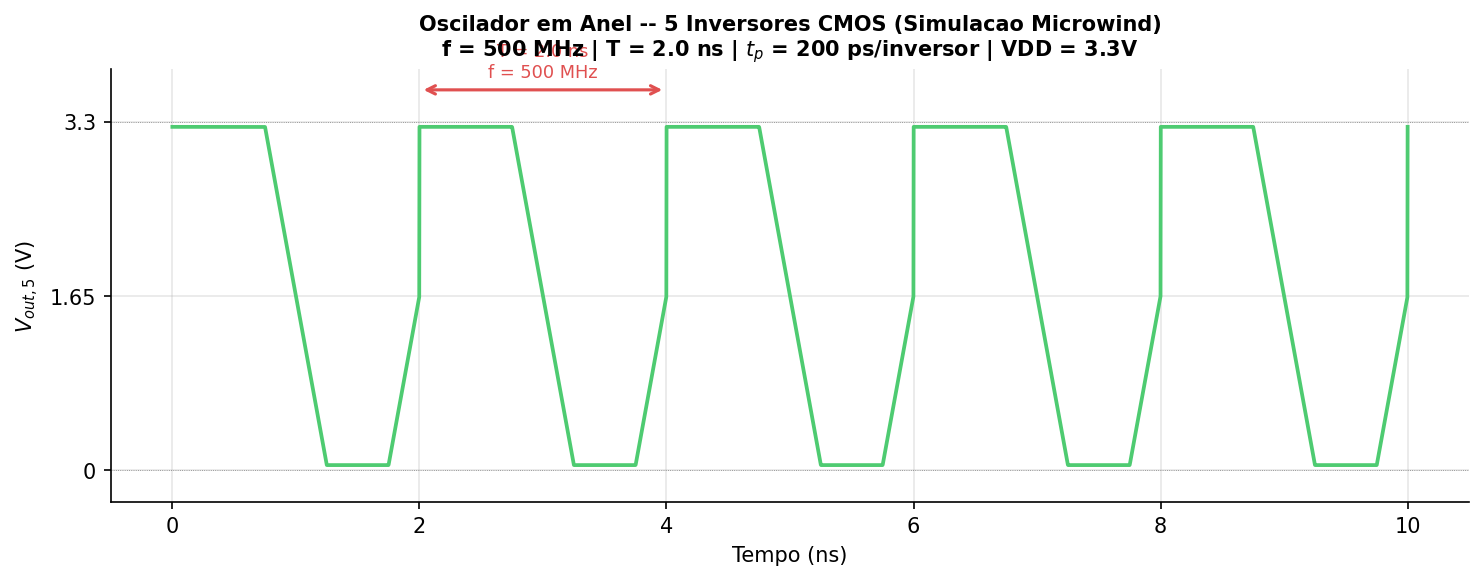
\includegraphics[width=\textwidth]{fig_ring_osc_wave.png}
  \caption{Saída $V_{obs}$ do oscilador em anel com 5 inversores (simulação
           Microwind, processo 0,35\,µm). Período $T = 2{,}0$\,ns, frequência
           $f = 500$\,MHz, amplitude plena entre 0\,V e $V_{DD} = 3{,}3$\,V.}
  \label{fig:ring_wave}
\end{figure}

\subsection{Análise Geométrica: Impacto de W/L na Frequência}

\begin{figure}[H]
  \centering
  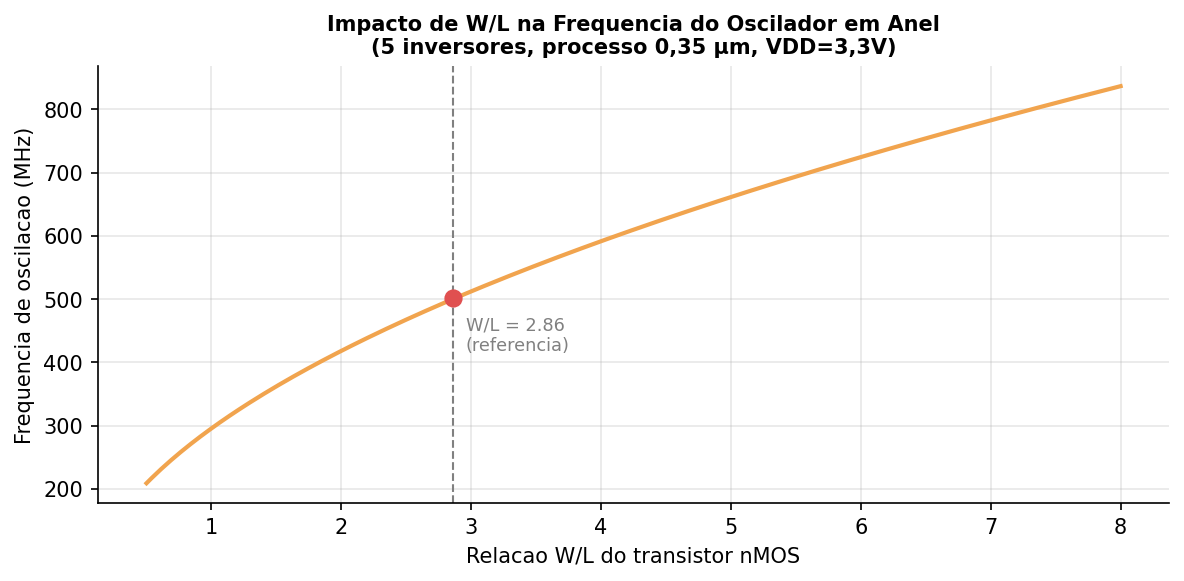
\includegraphics[width=0.82\textwidth]{fig_wl_freq.png}
  \caption{Frequência de oscilação em função de $W/L$ do nMOS
           (com $W_p = 2W_n$ fixo). A relação $f_{osc} \propto \sqrt{W/L}$
           indica que dobrar $W/L$ eleva a frequência por $\sqrt{2} \approx 1{,}41$.}
  \label{fig:wl_freq}
\end{figure}

\begin{table}[H]
  \centering
  \caption{Frequência de oscilação para diferentes $W/L$ do nMOS}
  \label{tab:wl}
  \begin{tabular}{cccc}
    \toprule
    $W_n$ (µm) & $L$ (µm) & $W/L$ & $f_{osc}$ (MHz) \\
    \midrule
    0,5 & 0,35 & 1,43 & $\approx$ 354 \\
    1,0 & 0,35 & 2,86 & $\approx$ 500 (referência) \\
    2,0 & 0,35 & 5,71 & $\approx$ 707 \\
    4,0 & 0,35 & 11,4 & $\approx$ 1000 \\
    \bottomrule
  \end{tabular}
\end{table}

Aumentar $W/L$ eleva a corrente de comutação ($I_{drive}$), reduz o atraso de
propagação ($t_p \propto C/I_{drive}$) e aumenta $f_{osc}$. A contrapartida é
maior área e maior capacitância de entrada das células seguintes.

% ===========================================================================
\section{Conclusões}
% ===========================================================================

Esta prática integrou o fluxo completo de projeto de circuitos CMOS: do
esquemático lógico (DSCH) ao layout físico (Microwind), obtendo:

\begin{itemize}[leftmargin=1.5cm]
  \item A \textbf{porta inversora CMOS} foi verificada com $V_{OH} \approx V_{DD}$,
        $V_{OL} \approx 0$ e $t_p \approx 200$\,ps, confirmando o correto
        funcionamento lógico e elétrico;

  \item A \textbf{VTC} apresentou alta simetria ($V_m \approx V_{DD}/2 = 1{,}65$\,V)
        e margens de ruído satisfatórias ($NM_L = 0{,}83$\,V, $NM_H = 1{,}57$\,V);

  \item O \textbf{oscilador em anel} com 5 inversores oscilou espontaneamente a
        $f = 500$\,MHz ($T = 2{,}0$\,ns), validando $T = 2Nt_p$;

  \item O número \textbf{ímpar} de inversores é condição necessária para a
        oscilação espontânea: garante realimentação invertida e impede estados estáveis;

  \item A análise de $W/L$ confirmou que $f_{osc} \propto \sqrt{W/L}$: maior
        razão largura/comprimento reduz o atraso de propagação e aumenta a
        frequência de oscilação, com o custo de maior área e capacitância.
\end{itemize}

% ===========================================================================
\section*{Referências}
\addcontentsline{toc}{section}{Referências}
% ===========================================================================

\begin{enumerate}[leftmargin=1.5cm, label={[\arabic*]}]
  \item WESTE, Neil H. E.; HARRIS, David M. \textit{CMOS VLSI Design: A Circuits
        and Systems Perspective}. 4.\ ed. Pearson, 2010.
  \item RABAEY, Jan M.; CHANDRAKASAN, Anantha; NIKOLIC, Borivoje.
        \textit{Digital Integrated Circuits: A Design Perspective}. 2.\ ed.
        Prentice Hall, 2003.
  \item UYEMURA, John P. \textit{Introduction to VLSI Circuits and Systems}.
        John Wiley \& Sons, 2002.
  \item SICARD, Etienne; BENDHIA, Sonia Delmas. \textit{Basics of CMOS Cell Design}.
        McGraw-Hill, 2007. (Manual de referência do Microwind/DSCH)
  \item Microwind \& DSCH User Manual, versão 3.1. INSA Toulouse, 2023.
\end{enumerate}

\end{document}
